\newappendix{Action-stability}\label{app:stable}

\vbstable*

\begin{proof}
Consider a datapoint $ z= (x,r)$ which becomes $ z(a) = (x, a, r(a))$ when we sample action $ a$ from the behavior. At this datapoint, the value-based objective for an estimated Q function $ \hat Q$ is
\begin{align}
    \ell(z(a), \hat Q(x, a)) = (r(a) - \hat Q(x,a))^2
\end{align}
This is minimized at all $ a $ by $\hat Q(x,a) = r(a)$. So setting $ y^* = \hat Q(x, \cdot) = r$, we can exactly minimize $ \ell$ at $ z$. Since such a $ y^*$ exists, the objective is by definition action-stable.
\end{proof}



\pbstable*

\begin{proof}
Consider a datapoint $ z= (x,r)$ which becomes $ z(a) = (x, a, r(a), p(a))$ when we sample action $ a$ from the behavior with probability $ p(a)$. At this datapoint, a generic policy-based objective evaluated on a policy $ \hat \pi $ takes the form
\begin{align}
    \ell(z(a), \hat \pi(a|x)) = f(z(a)) \hat \pi(a|x)
\end{align}
As special examples of the function $ f $ we have the generic policy-based objective from Equation (\ref{eq:pi}) when $ f(z(a)) = \frac{r(a)}{p(a)}$. Moreover we can incorporate any baseline function $ b(x)$ so that $ f(z(a)) = \frac{r(a) - b(x)}{p(a)}$. This algorithm covers the one presented by \citet{joachims2018deep}.

Now to prove the claim, we have three cases: (1) $ f(z(a)) < 0$ for all $ a$, (2) $ f(z(a)) > 0 $ for at least two actions $ a_1, a_2$, and (3) $ f(z(a)) > 0$ at exactly one action $ a_1$. We will show that in cases 1 and 2 the objective is action-unstable, but in case 3 it is action-stable.

\paragraph{Case 1.} Assume that $ f(z(a)) < 0$ for all $ a$. Now for any given $ a $ to maximize the objective $f(z(a))\hat \pi(a|x)$ while ensuring that $ \hat \pi(a|x) $ is a valid probability we must set $ \hat \pi(a|x) = 0$. But, if we set $ \hat\pi(a|x) = 0$ for all $ a$, we no longer have a valid probability distribution, since $ 0 \not \in \Delta^K$. Thus, we cannot find $ y^* \in \Delta^K$ that optimizes the loss at $ z $ across all actions, so the objective is action-unstable.

\paragraph{Case 2.} Assume that $ f(z(a)) > 0 $ for at least two actions $ a_1, a_2$. Now at $ a_1, a_2$ the objective $f(z(a))\hat \pi(a|x)$ is maximized by setting $ \pi(a|x) = 1$. However, there is no valid element $ y $ of $ \Delta^K$ such that $ y(a_1) = 1$ and $y(a_2) = 1$. Thus, we cannot find $ y^* \in \Delta^K$ that optimizes the loss at $ z $ across all actions, so the objective is action-unstable.

\paragraph{Case 3.} Assume $f(z(a)) > 0$ at exactly one action $ a_1$. Then at action $ a_1$ we can maximize $ f(z(a_1))\hat \pi(a_1|x)$ by setting $ \hat\pi(a_1|x) = 1$. And since $ f(z(a)) \leq 0$ for all other actions $ a \neq a_1$, we can maximize $ f(z(a))\hat \pi(a|x)$ by setting $ \hat\pi(a|x) = 0$. Now since $ \one[a = a_1] \in \Delta^K$, there does exist a vector $ y^* \in \mathcal{Y}$ which exactly optimizes $ \ell$ regardless of which action is sampled. So, the objective is action-stable if and only if we are in this case.
\end{proof}




\newappendix{Value-based learning}\label{app:value}

\reduction*

\begin{proof}
The proof follows directly from linking the subsequent lemmas with $ \hat \pi = \pi_{\hat Q_{S_B}}$ and $ \Pi$ be the set of all policies in Lemma \ref{lem:mismatch}.
\end{proof}


% \paragraph{Mismatch.} We need to connect the bound on worst case the regression error to the value of the learned policy. This follows from some algebraic manipulation and an application of Jensen's inequality and is encoded in the following Lemma.

\begin{restatable}[Mismatch: from MSE to Regret]{lemma}{mismatch}\label{lem:mismatch}
Assume strict positivity. Let $\hat \pi$ be the greedy policy with respect to some $ \hat Q $ and let $ \Pi$ be any class of policies to compete against, which contains $ \hat \pi$. Then
\begin{align}
    \sup_{\pi\in \Pi} V(\pi) - V(\hat\pi) \leq 2 \sqrt{\sup_{\pi\in \Pi} \E_{x,a \sim \mathcal{D}, \pi}[ (Q(x,a) - \hat Q(x,a))^2]}
\end{align}
\end{restatable}


\begin{proof}
We can expand the definition of regret and then add and subtract and apply a few inequalities. Let $ \bar \pi $ be the policy in $ \Pi $ which maximizes $ V$. Then
\begin{align}
    \sup_{\pi\in \Pi}V(\pi) - V(\hat \pi) &=  \E_x\bigg[\E_{a\sim \bar\pi|x}[Q(x,a)] - \E_{a\sim\hat\pi|x}[Q(x,a)]\bigg]\\
    &= \E_x\bigg[\E_{a\sim \bar\pi|x}[ Q(x,a)] - \E_{a\sim\hat\pi|x}[\hat Q(x,a)] + \E_{a\sim\hat\pi|x}[\hat Q(x,a)] - \E_{a\sim\hat\pi|x}[Q(x,a)]\bigg]\\
    &\leq \E_x\bigg[\E_{a\sim \bar\pi|x}[| Q(x,a) -\hat Q(x,a)|] + \E_{a\sim\hat\pi|x}[|Q(x,a)-\hat Q(x,a)|]\bigg]\\
    &\leq \sqrt{\E_x\E_{a\sim \bar\pi|x}[(Q(x,a) -\hat Q(x,a))^2]} + \sqrt{\E_x\E_{a\sim \hat\pi|x}[(Q(x,a) -\hat Q(x,a))^2]} \\
    &\leq 2  \sqrt{ \sup_{\pi\in \Pi}\E_x\big[\E_{a\sim \pi|x}[(Q(x,a)-  \hat Q(x,a))^2]\big]}
\end{align}
The first inequality holds since $ \hat \pi $ maximizes $ \hat Q$ and by using the definition of absolute value, the second by Jensen, and the third by introducing the supremum.
\end{proof}

\begin{restatable}[Transfer: from $\beta$ to $\pi$]{lemma}{transfer}\label{lem:transfer}
Assume strict positivity and take any Q-function $ \hat Q $ and any policy $ \pi$, then
\begin{align}
    \E_{x, a\sim \mathcal{D}, \pi}[Q(x,a) - \hat Q(x,a))^2] < \frac{1}{\tau}\bigg(\E_{x,a \sim \mathcal{D}, \beta}[(Q(x,a) - \hat Q(x,a))^2]\bigg).
\end{align}
\end{restatable}
\begin{proof} Let $ \pi$ be any policy. Then
\begin{align}
    \E_{x}\E_{a\sim \pi|x} [(Q(x,a) - \hat Q(x,a))^2] &=  \int_x p(x) \sum_a \pi(a|x) (Q(x,a) - \hat Q(x,a))^2 dx \\
    &=  \int_x \sum_a \pi(a|x) \frac{\beta(a|x)}{\beta(a|x)} p(x) (Q(x,a) - \hat Q(x,a))^2 dx \\
    &<  \frac{1}{\tau}\int_x \sum_a \beta(a|x) p(x) (Q(x,a) - \hat Q(x,a))^2 dx\\
    &= \frac{1}{\tau} \E_{x,a \sim \mathcal{D}, \beta}[(Q(x,a) - \hat Q(x,a))^2]
\end{align}
where we use a multiply and divide trick and apply the definition of strict positivity to ensure that $ \frac{\pi(a|x)}{\beta(a|x)} < \frac{1}{\tau}$.
\end{proof}


\newappendix{Policy-based learning}\label{app:pb}


\subsection{In-sample regret}



\begin{lemma}\label{lem:policy_decomp}
Let $ \Pi$ be an interpolating class and $ K = 2$. Then there exists a $ \pi_B $ as defined in Equation (\ref{eq:pi}) such that
\begin{enumerate}
    \item the behavior of $ \pi_B$ at each datapoint $ x_i \in S$ only depends on $ a_i, r_i(a_i)$, and $ p_i$
    \item $ \pi_B(\cdot|x_i) \in \{(0,1),(1,0)\}$.
\end{enumerate}
\end{lemma}
\begin{proof}
We will begin by proving part 2. Note that the objective that $ \pi_B$ optimizes takes the form $ \frac{r_i(a_i)}{p_i}\pi(a_i|x_i)$ at each datapoint. Since probabilities are constrained to $[0,1]$ this is optimized by $ \pi(a_i|x_i) = 0$ if $ \frac{r_i(a_i)}{p_i} < 0$ and $ \pi(a_i|x_i) = 1$ if $ \frac{r_i(a_i)}{p_i} > 0$. Since we have an overparameterized model class, we know that $ \Pi$ contains a $ \pi_B$ that can exactly choose the optimizer at each datapoint. Since $ K=2$, once we know $ \pi(a_i|x_i)$ we immediately have $ \pi(\bar a_i|x_i) = 1 - \pi(a_i|x_i)$ (where $ \hat a_i$ is the action that is not equal to $ a_i$). Thus $ \pi_B(\cdot|x_i) \in \{(0,1),(1,0)\}$.

Now part 1 follows directly since the above reasoning showed that $ \pi_B(\cdot|x_i)$ is defined precisely by the sign of $ \frac{r_i(a_i)}{p_i}$ and the identity of $ a_i$.
\end{proof}



\vsthm*

\begin{proof}
By part 1 of Lemma \ref{lem:policy_decomp} and linearity of expectation we can decompose the expected in-sample value as
\begin{align*}
    \E_{S}[V(\pi^*;S) - V(\pi_B;S)] = \frac{1}{N}\sum_{i=1}^N \E_{x_i, r_i, a_i}\bigg[ \E_{a\sim \pi^*}\E_{r|x_i}[r(a)] -  \E_{a\sim \pi_B}\E_{r|x_i}[r(a)]\bigg].
\end{align*}

Since the data are iid we further have that
\begin{align*}
    \E_{S}[V(\pi^*;S) - V(\pi_B;S)] = \E_{x_i, r_i, a_i}\bigg[ \E_{a\sim \pi^*}\E_{r|x_i}[r(a)] -  \E_{a\sim \pi_B}\E_{r|x_i}[r(a)]\bigg].
\end{align*}

Define the event $ U_{x,r}$ to be the event that the policy-based objective is action-unstable at $ x,r$. So $ p_u(x) = \E_{r|x}[\one[U_{x,r}]]$.
We can split this expectation up into stable and unstable parts by conditioning on either $ \overline U_{x_i, r_i}$ or $ U_{x_i, r_i}$, and lower bound the regret on the stable datapoints by 0:
\begin{align*}
    \E_{S}[V(\pi^*;S) - V(\pi_B;S)] &= \E_{x_i, r_i |\overline U_{x_i, r_i}} \E_{a_i|x_i}\bigg[ \E_{a\sim \pi^*}\E_{r|x_i}[r(a)] -  \E_{a\sim \pi_B}\E_{r|x_i}[r(a)]\bigg] \\
    &\qquad + \E_{x_i, r_i |U_{x_i, r_i}} \E_{ a_i|x_i}\bigg[ \E_{a\sim \pi^*}\E_{r|x_i}[r(a)] -  \E_{a\sim \pi_B}\E_{r|x_i}[r(a)]\bigg]\\
    &\geq \E_{x_i, r_i |U_{x_i, r_i}} \E_{ a_i|x_i}\bigg[ \E_{a\sim \pi^*}\E_{r|x_i}[r(a)] -  \E_{a\sim \pi_B}\E_{r|x_i}[r(a)]\bigg].
\end{align*}

By part 2 of Lemma \ref{lem:policy_decomp} we know that $ \pi_B(\cdot|x_i) $ is either $ (1,0)$ or $ (0,1)$. Conditioned on the objective being unstable at $ x_i$ and using the fact that there are only two actions, we know that $ \pi_B(x_i)$ must be different depending on whether $ a_i = 1$ or $ a_i = 2$. Define $ a_{i,B}^1$ to be the action that $ \pi_B$ selects at $ x_i $ when $ a_i = 1$ and $ a_{i,B}^2$ the action when $ a_i = 2$.
Let $ a_i^*$ be the action chosen by the deterministic optimal policy $ \pi^*$ at $ x_i$.
Thus we can split the expectation over $ a_i$ in the above expression and then plug in definitions to get:
\begin{align*}
    \E_{S}[V(\pi^*;S) - V(\pi_B;S)] &\geq \E_{x_i, r_i |U_{x_i, r_i}} \bigg[\beta(a_i = 1|x_i) \E_{r|x_i}[r(a^*_i) - r(a_{i,B}^1)] + \beta(a_i = 2|x_i) \E_{r|x_i}[r(a^*_i) - r(a_{i,B}^2)]\bigg].
\end{align*}
Since we assumed that $ \beta (a|x_i) \geq \tau$ for all $ a$ we can lower bound the above by
\begin{align*}
    \E_{S}[V(\pi^*;S) - V(\pi_B;S)] &\geq \tau \E_{x_i, r_i} \bigg[\one[U_{x_i, r_i}]\bigg( \E_{r|x_i}[r(a_i^*) - r(a_{i,B}^1)] +  \E_{r|x_i}[r(a_i^*) - r(a_{i,B}^2)]\bigg)\bigg].
\end{align*}
Finally, we note that since $ a_{i,B}^1 \neq a_{i,B}^2$ and there are only 2 actions that the above is precisely
\begin{align*}
    \E_{S}[V(\pi^*;S) - V(\pi_B;S)] &\geq  \tau \E_{x_i, r_i} \bigg[\one[\overline E_{x_i, r_i}] \E_{r|x_i}[r(a_i^*) - r(a \neq a^*_i)]\bigg]\\
    &= \tau \E_{x_i, r_i} [\one[\overline E_{x_i, r_i}] \Delta_r(x_i)]\\
    &= \tau \E_{x_i} [\E_{r_i|x_i}[\one[U_{x_i, r_i}]] \Delta_r(x_i)]\\
    &= \tau \E_{x_i} [p_u(x_i) \Delta_r(x_i)]\\
    &= \tau \E_{x} [p_u(x) \Delta_r(x)].
\end{align*}
\end{proof}



\subsection{Connection to noisy classification}\label{app:noisy}

This section states and proves the Theorem referenced in the main text connecting action-unstable policy-based learning with noisy classification.

%\noisy*
\begin{restatable}[Noisy classification reduction]{theorem}{noisy}\label{thm:noisy}
Take any noise level $ \eta < 1/2$ and any binary classification problem $ \mathcal{C}$ consisting of a distribution $\mathcal{D}_\mathcal{C}$ over $ \mathcal{X}$ and a labeling function $ y_{\mathcal{C}}: \mathcal{X} \to \{-1,1\}$.
There exists an offline contextual bandit problem $ \mathcal{B}$ with noiseless rewards such that
\begin{enumerate}
    \item Maximizing $ \hat V_B$ in $\mathcal{B}$ is equivalent to minimizing the 0/1 loss on a training set drawn from $ \mathcal{C}$ where labels are flipped with probability $ \eta$.
    \item Maximizing $ \hat V_F$ in $\mathcal{B}$ is equivalent to minimizing the 0/1 loss on a training set drawn from $ \mathcal{C}$ with noiseless training labels.
\end{enumerate}
\end{restatable}

\begin{proof}
First we will construct the bandit problem $ \mathcal{B}$ with two actions corresponding to the classification problem $ \mathcal{C}$.
For any constant $ c_r > 0 $ we define $ \mathcal{B}$ by
\begin{align}
    x \sim \mathcal{D}_{\mathcal{C}}, \qquad r|x = \begin{cases}c_r(1-\eta, \eta) & y_\mathcal{C}(x) = 1\\ c_r(\eta, 1-\eta) & y_\mathcal{C}(x) = -1\end{cases}, \qquad \beta(1|x) = \begin{cases}1-\eta & y_\mathcal{C}(x) = 1\\ \eta & y_\mathcal{C}(x) = -1\end{cases}
\end{align}
Now we will show that in this problem, $ \hat V_B$ is equivalent to the 0/1 loss for $ \mathcal{C}$ with noisy labels. To do this first note that by construction, for $ x $ with $ y_\mathcal{C}(x) = 1$ we have $ \frac{r(1)|x}{\beta(1|x)} = \frac{c_r(1-\eta)}{1-\eta} = c_r$ and $ \frac{r(2)|x}{\beta(2|x)} = \frac{c_r\eta}{\eta} = c_r$, and similarly for $ x $ with $ y_\mathcal{C}(x) = -1$ we have $ \frac{r(1)|x}{\beta(1|x)} = \frac{c_r\eta}{\eta} = c_r$ and $ \frac{r(2)|x}{\beta(2|x)} = \frac{c_r(1-\eta)}{1-\eta} = c_r$.
\begin{align}
    \hat V_B(\pi) &= \frac{1}{N} \sum_{i=1}^N r_i(a_i) \frac{\pi(a_i|x_i)}{\beta(a_i|x_i)} = \frac{1}{N} \sum_{i=1}^N  \frac{r_i(a_i)}{\beta(a_i|x_i)} \pi(a_i|x_i) \\
    &= \frac{c_r}{N} \sum_{i=1}^N  \pi(a_i|x_i)
\end{align}
This is equivalent to 0/1 loss with noisy labels since $ \beta$ generates $ a_i$ according to $ y_\mathcal{C}$ where the label is flipped with probability $ \eta$.

Now we will show that $ \hat V_F$ is equivalent to the 0/1 loss for $ \mathcal{C}$ with clean labels. Note that by construction $ r(a)|x = c_r \eta + \pi^*(a|x)c_r (1 - 2 \eta)$. So,
\begin{align}
    \hat V_F(\pi) &= \frac{1}{N} \sum_{i=1}^N \langle r_i, \pi(\cdot|x_i)\rangle = \frac{c_r}{N} \sum_{i=1}^N \langle \eta \textbf{1} + (1 - 2\eta) \pi^*(\cdot|x_i), \pi(\cdot|x_i)\rangle \\
    &= \frac{c_r \eta}{N} +  \frac{c_r (1 - 2\eta)}{N} \sum_{i=1}^N \langle  \pi^*(\cdot|x_i), \pi(\cdot|x_i)\rangle
\end{align}
This is equivalent to 0/1 loss with noisy labels since $ \pi^*$ exactly corresponds to $ y_\mathcal{C}$.
\end{proof}





\subsection{Nearest Neighbor}

\nn*

\begin{proof}
First we need to formally define the nearest neighbor rules that interpolate the objectives $ \hat V_B$ and $ \hat V_F$. These are simple in the case of two actions. Let $ i(x)$ be the index of the nearest neighbor to $ x$ in the dataset. Then
\begin{align}
    \pi_B(a|x) = \begin{cases}1 & \big(a = a_{i(x)} \ \textsc{and}\  r_{i(x)}(a_{i(x)}) > 0\big) \textsc{or} \big(a \neq a_{i(x)} \ \textsc{and}\  r_{i(x)}(a_{i(x)}) \leq 0\big) \\ 0 & otherwise.\end{cases}
\end{align}
This is saying that $ \pi_B$ chooses the same action as the observed nearest neighbor if that reward was positive, and the opposite action if that was negative.
And for the full feedback we just choose the best action from the nearest datapoint.
\begin{align}
    \pi_F(a|x) = \begin{cases}1 & a = \arg\max_{a'} r_{i(x)}(a')\\ 0 & otherwise. \end{cases}
\end{align}

Now we can construct the problem instances needed for the Theorem.
To construct the example, take a bandit problem with two actions (called 1 and 2):
\begin{align*}
    x \sim U([-1,1]), \quad r|x = (1, 1 + \Delta_r), \quad \beta(1|x) = \beta(2|x) = 1/2 \ \forall\ x,a
\end{align*}
The true optimal policy has $\pi^*(2|x) = 1$ for all $x$ and $ V(\pi^*) = 1+\Delta_r$.
The policy with full feedback $ \pi_F $ is to always choose action 2, since every observation will show that action 2 is better.


Now, we will show that in the limit of infinite data, $ \pi_F$ has no regret. Since the rewards are noiseless, the maximum observed reward at a context is exactly the optimal action at that context. Thus, we precisely have a classification problem with noiseless labels so that the Bayes risk is 0.
Since we $\pi^*$ is continuous, the class conditional densities (determined by the indicator of the argmax of $ Q$) are piecewise continuous.
This allows us to apply the classic result of \cite{cover1967} that a nearest neighbor rule has asymptotic risk less twice the Bayes risk, which in this case is zero. This means that asymptotically $ P(\pi_F(a|x) \neq \pi^*(a|x)) = 0$ which immediately gives the second desired result of zero regret in the limit of infinite data under full feedback.

Now we note that since rewards are always positive, we can simplify the definition of $ \pi_B$ as
\begin{align}
    \pi_{B}(a|x) = \one[a = a_{i(x)}].
\end{align}

Then we have that
\begin{align}
    V(\pi_F) - V(\pi_{B}) &= \E_x [\E_{a\sim \pi_F|x}[Q(x,a)] - \E_{a\sim \pi_{B}|x}[Q(x,a)] ]\\
    &= \E_x [\Delta_r + 1 - (\pi_{B}(1|x) + \pi_{B}(2|x) (\Delta_r + 1))] ] \\
    &= \Delta_r + 1 - \E_x[\one[a_{i(x)} = 1] + (\Delta_r + 1)\one[a_{i(x)} = 2]]
\end{align}
Taking expectation over $ S$ we get
\begin{align}
    \E_S[V(\pi_F) - V(\pi_{B})] &= \E_S[\Delta_r + 1 - \E_x[\one[a_{i(x)} = 1] + (\Delta_r + 1)\one[a_{i(x)} = 2]]]\\
    &= \Delta_r + 1 - \E_x[P_S(a_{i(x)} = 1) + (\Delta_r + 1)P_S(a_{i(x)} = 2)]]\\
    &= \Delta_r + 1 - \E_x[\frac{1}{2} + (\Delta_r + 1)\frac{1}{2}]]\\
    &= \frac{\Delta_r}{2}
\end{align}
This construction did not depend on the size of the dataset, so it is even true as the number of datapoints tends to infinity.
\end{proof}



\newappendix{Discussion of doubly robust algorithms}\label{app:dr}


Before going into the comparison, we will define the doubly robust algorithm \cite{dudik2011doubly} in our notation. Specifically,
\begin{align}\label{eq:dr}
    \widehat V_{DR} (\pi) := \sum_{i=1}^N \bigg[ \sum_a \pi(a|x_i) \hat Q(x_i, a) + \frac{\pi(a_i|x_i)}{\beta(a_i|x_i)} (r_i(a_i) - \hat Q(x_i, a_i)) \bigg], \qquad \hat \pi_{DR} = \arg\max_{\pi \in \Pi} \widehat V_{DR}(\pi)
\end{align}

As stated in the main text, when we use overparameterized models and train $ \hat Q$ on the same data that we use to optimize the policy, then doubly robust methods are equivalent to the vanilla value-based algorithm. This is formalized in Lemma \ref{lem:dr_equiv} below.

This equivalence can be avoided by using crossfitting so that $ \hat Q$ is not trained on the same data as $ \pi$. However, then it is possible that the doubly robust policy objective becomes action-unstable. This is true \emph{even with} access to the true $Q$ function, but requires stochastic rewards. To construct such an example we leverage the stochastic rewards so that instability only occurs at datapoints where certain reward vectors are sampled. This is shown in Lemma \ref{lem:dr_unstable} below.

One final point is to consider the motivation for doubly robust methods. Usually it is motivated by concerns about consistency of the value function estimation or estimation of behavior policy \cite{dudik2011doubly}. However, in our setting we have (1) an overparamterized model class which is large enough to contain the true value function, and (2) exact access to the behavior probabilities. So it is not clear why doubly robust methods would be motivated in our setting.

\begin{lemma}[Equivalence of DR and vanilla VB]\label{lem:dr_equiv}
When we use overparameterized models and do not use crossfitting, doubly robust learning from Equation (\ref{eq:dr}) is equivalent to vanilla value-based learning from Equation (\ref{eqn:hatQ}).
\end{lemma}

\begin{proof}
When the model for $ \hat Q$ is overparameterized and trained on the full dataset, we know that $ \hat Q(x_i, a_i) = r_i(a_i)$. Thus we get that
\begin{align}
    \widehat V_{DR} (\pi) &= \sum_{i=1}^N \bigg[ \sum_a \pi(a|x_i) \hat Q(x_i, a) + \frac{\pi(a_i|x_i)}{\beta(a_i|x_i)} (r_i(a_i) - \hat Q(x_i, a_i)) \bigg]\\
    &= \sum_{i=1}^N \bigg[ \sum_a \pi(a|x_i) \hat Q(x_i, a) + \frac{\pi(a_i|x_i)}{\beta(a_i|x_i)} (0) \bigg]\\
    &= \sum_{i=1}^N \sum_a \pi(a|x_i) \hat Q(x_i, a)
\end{align}
With an overparameterized policy class, we can exactly recover the greedy policy relative to $ \hat Q$ to optimize this objective.
\end{proof}


\begin{lemma}[Instability of DR]\label{lem:dr_unstable}
There exist problems with stochastic rewards where even with access to the exact Q function, the doubly robust policy objective is action-unstable with probability 1/2.
\end{lemma}

\begin{proof}
We need only consider one datapoint since the action-stability property is defined on a per datapoint basis. To make this construction we will consider only two actions.
\begin{align}
    r|x = \begin{cases} (0, 1) & w.p.\ 1/2\\ (0, -2) & otherwise\end{cases}, \qquad \beta(\cdot|x) = (1/2, 1/2)
\end{align}
So, we know that
\begin{align}
    Q(\cdot|x) = (0,-0.5)
\end{align}
Now we claim that when the sampled datapoint has $ r = (0,1)$ the doubly robust objective is action-unstable (and this happens with probability 1/2 by construction).
We can explicitly expand the DR objective for the policy $ \pi$ at $ x $ when action $ a $ is sampled
\begin{align}
    \ell_{DR}(\pi, x, a, r) = \pi(1|x) \cdot 0 + \pi(2|x) \cdot (-0.5) + \frac{\pi(a|x)}{1/2}(r(a) - Q(x,a))
\end{align}
So when $a = 1$ we have $ r(a) = 0$ and $ Q(x,a) = 0$ so that
\begin{align}
    \ell_{DR}(\pi, x, a, r) = \pi(2|x) \cdot (-0.5) + 2 \cdot \pi(1|x)(0 - 0) = \pi(2|x) \cdot (-0.5)
\end{align}
And when $ a=2$ we have $ r(a) = 1$ (because that was the sampled reward) and $ Q(x,a) = 0$ so that
\begin{align}
    \ell_{DR}(\pi, x, a, r) = \pi(2|x) \cdot (-0.5)  + 2 \cdot \pi(2|x) (1 - (-0.5)) = \pi(2|x) \cdot (2.5)
\end{align}
Now, this is clearly action-unstable since the optimizer when $ a=1 $ is sampled is $ \pi(\cdot|x) = (1,0)$ while when $ a = 2$ is sampled we get $ \pi(\cdot|x) = (0,1)$.
\end{proof}





\newappendix{Details of Bandit Experiments}\label{app:experiments}

\subsection{Synthetic data}

\paragraph{Data.} As described in the main text we sample some hidden reward matrix $ \theta$ and then sample contexts and rewards from isotropic Gaussians:
\begin{align*}
    \theta \sim U([0,1]^{K\times d}),\quad x \sim \mathcal{N}(0, I_d), \quad r \sim \mathcal{N}(\theta x, \epsilon I_d).
\end{align*}
Actions are sampled according to a uniform behavior:
\begin{align*}
    a\sim \beta(\cdot|x) = U(\{1,\dots,K\}).
\end{align*}
We set $ K=2, d = 10, \epsilon = 0.1$. For each random seed we take $ N = 100$ training points and sample an independent test set of 500 points.
For experiment 1 we sample $ \theta$ and one dataset of $ x,r$ tuples, then we sample 20 independent sets of actions. For experiment 2 we sample all parameters separately to construct each of the 50 datasets.

\paragraph{Model.} For policies and Q functions we use a multilayer perceptron with one hidden layer of width 512 and ReLU activations. The only difference between policy and Q architecture is that the policy has a softmax layer on the output so that the output is a probability distribution.

\paragraph{Learning.} We train using SGD with momentum. Learning rate is 0.01, momentum is 0.9, batch size is 10, and weight decay is 0.0001. We train every model for 1000 epochs decreasing the learning rate by a factor of 10 after 200 epochs. This trains well past the point of convergence in our experience.

\begin{figure}[h]
    \centering
    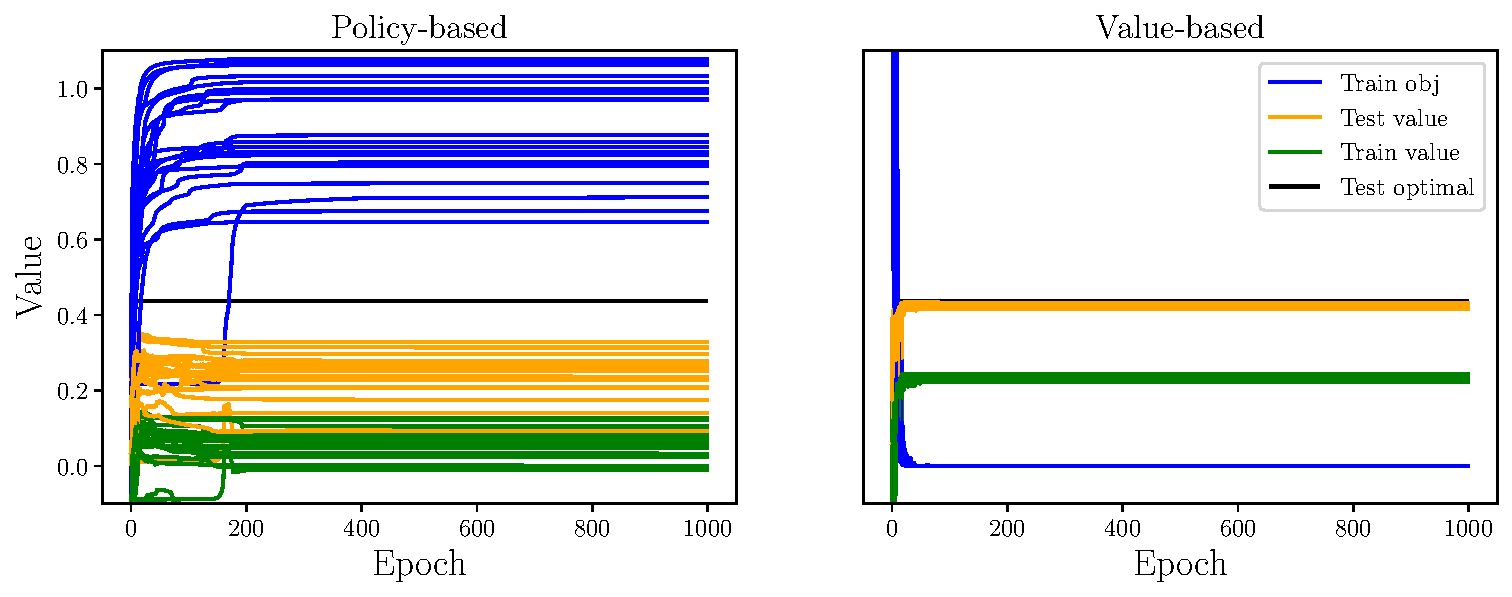
\includegraphics[width=0.7\textwidth]{figures/offline-bandits/toy_learning.pdf}
    \caption{We show learning curves across each of the twenty different action resampled datasets.}
    \label{fig:toy_learning}
\end{figure}

\paragraph{Extended results.}
Figure \ref{fig:toy_learning} shows learning curves for each of the twenty different action datasets from experiment 1. We use ``train obj'' to refer to the training objective which is squared error for value-based learning and $ \hat V_B$ for policy-based learning. We use ``train value'' and ``test value'' to refer to  $ V(\pi;S)$ for $ S$ being the train and test sets respectively. We can evaluate the true value at each datapoint since we know the full reward vector at each datapoint.

We see that the policy-based objective is dramatically higher than the highest achievable value due to overfitting of the noise in the actions. The gap between train and test value is mot likely explained by noise in the contexts sampled in those respective datasets (by chance the test set has higher value contexts).



\subsection{CIFAR-10}

\paragraph{Data.} We use a bandit version of the CIFAR-10 dataset \citep{Krizhevsky09learningmultiple}. We split the train set into a train set of the first 45000 examples and validation set of the last 5000. We normalize the images and use data augmentation of random flips and crops of size 32. Each of the 10 labels becomes an action. We define rewards to be 1 for a correct prediction and 0 for an incorrect prediction.
We use two different behavior policies. One is a uniform behavior that selects each action with probability 0.1 and the other is the hand-crafted behavior policy from \cite{joachims2018deep}.

\paragraph{Model.} We use a ResNet-18 \citep{he2016deep} from PyTorch \citep{paszke2019pytorch} for both the policy and the Q function. The only modification we make to accommodate for the smaller images in CIFAR is to remove the first max-pooling layer.

\paragraph{Learning.} We train using SGD with momentum 0.9,a batch size 128, and weight decay of 0.0001 for 1000 epochs. Training takes about 20 hours for each run on an NVIDIA RTX 2080 Ti GPU. We use a learning rate of 0.1 for the first 200 epochs, 0.01 for the next 200, and 0.001 for the last 600. To improve stability we use gradient clipping and reduce the learning rate in the very first epoch to 0.01.

\paragraph{Extended results.}
Figures \ref{fig:cifar_learning_blbf} and \ref{fig:cifar_learning_uniform} show learning curves for each of the three algorithms we consider across each dataset. The labels refer to the same quantities as they did on the synthetic problem.

One interesting phenomena is that the unstable policy-based algorithm displays a clear overfitting phenomena as we would predict due to the noise in the actions being transferred into noise in the objective. Since we have strictly positive rewards here, this is also an instance of ``propensity overfitting'' \cite{swaminathan2015self}. As a result, limiting the capacity of the model class by early stopping could improve performance somewhat. But by limiting capacity in this way we are exiting the overparameterized/interpolating regime described by \citet{zhang2016understanding}.

\begin{figure}[h]
    \centering
    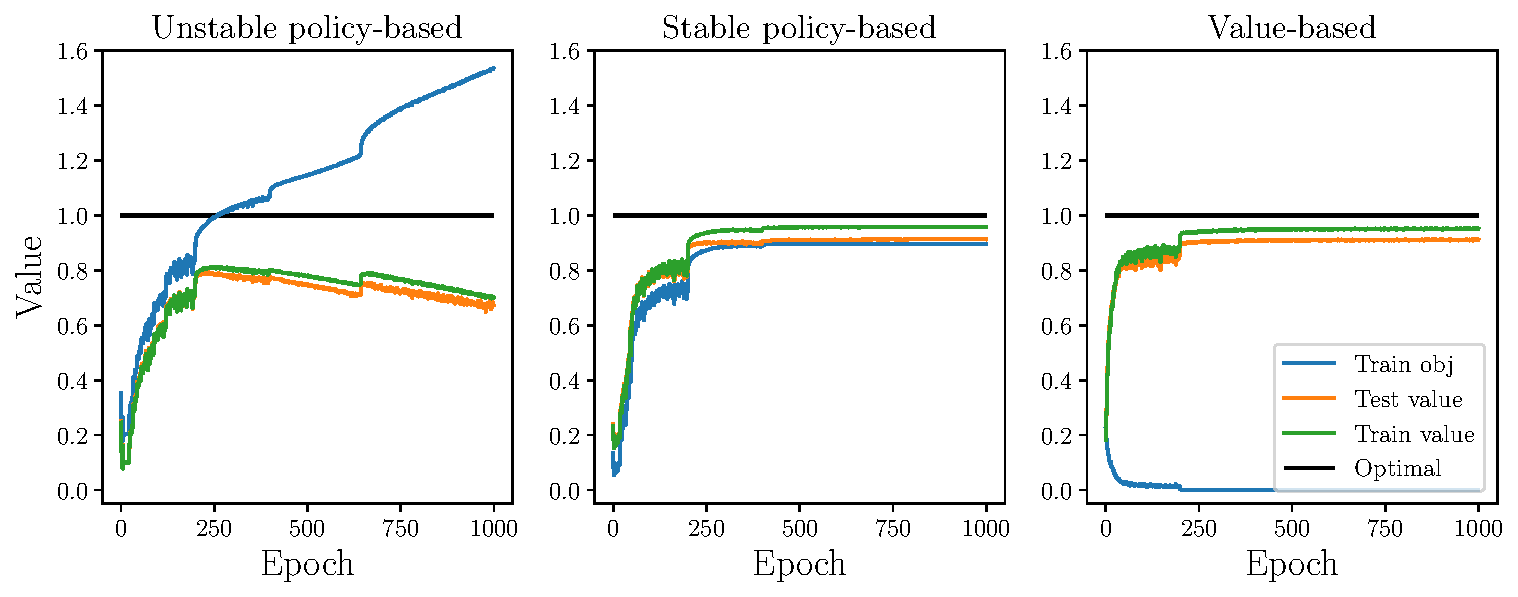
\includegraphics[width=0.7\textwidth]{figures/offline-bandits/cifar_learning_blbf.pdf}
    \caption{Learning curves on the hand-crafted action dataset.}
    \label{fig:cifar_learning_blbf}
\end{figure}


\begin{figure}[h]
    \centering
    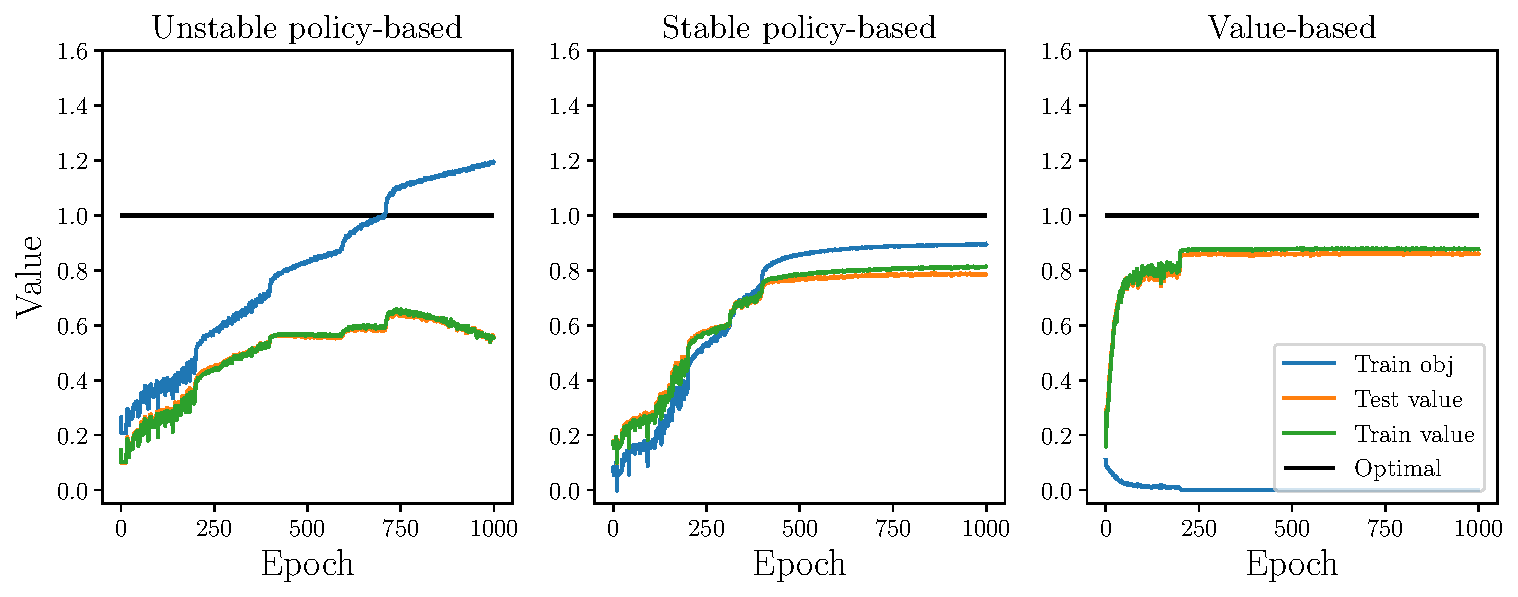
\includegraphics[width=0.7\textwidth]{figures/offline-bandits/cifar_learning_uniform_0.pdf}
    \caption{Learning curves on the uniform action dataset.}
    \label{fig:cifar_learning_uniform}
\end{figure}



\newappendix{Small model classes}\label{app:small}


In this section we state and prove theorems that bound each term of our regret decomposition for each algorithm we consider when we use finite model classes. Similar results can be shown for other classical notions of model class complexity. We include these results for completeness, but the main focus of our paper is the overparameterized regime where such bounds are vacuous.


\begin{theorem}[Policy-based learning with a small model class]\label{thm:pol-small}
Assume strict positivity and a finite policy class $ \Pi$. Let $ \varepsilon_\Pi = V(\pi^*) - \sup_{\pi \in \Pi} V(\pi)$. Denote $ \Delta_r = r_{max} - r_{min}$. Then we have that for any $ \delta > 0$ with probability $ 1- \delta$ each of the following holds:
\begin{align*}
    \text{Approximation Error} &= V(\pi^*) - \sup_{\pi\in \Pi}V(\pi) \leq \varepsilon_\Pi\\
    \text{Estimation Error}  &= \sup_{\pi\in \Pi}V(\pi) - V(\pi_F) \leq 2\Delta_r \sqrt{\frac{\log(2|\Pi|/\delta)}{2N}}\\
    \text{Bandit Error}  &= V(\pi_F) - V(\pi_B) \leq \frac{2\Delta_r}{\tau} \sqrt{\frac{\log(2|\Pi|/\delta)}{2N}}
\end{align*}
\end{theorem}
\begin{proof}
The bound on approximation error follows directly from the definition of $ \varepsilon_\Pi$. The bound on the estimation error follows from a standard application of a Hoeffding bound on the random variables $ X_i = \langle r_i, \pi(\cdot|x_i)\rangle
$ which are bounded by $ \Delta_r$ and a union bound over the policy class.

The bound on bandit error essentially follows Theorem 3.2 of \cite{strehl2010learning}, we include a proof for completeness:
\begin{align*}
    V(\pi_F) - V(\pi_B) &= V(\pi_F) - \hat V_B(\pi_B) + \hat V_B(\pi_B) - V(\pi_B) \\
    &\leq V(\pi_F) - \hat V_B(\pi_F) + \hat V_B(\pi_B) - V(\pi_B)\\
    &\leq 2 \sup_{\pi \in \Pi} |V(\pi) - \hat V_B(\pi)|\\
    &\leq \frac{2\Delta_r}{\tau} \sqrt{\frac{\log(2|\Pi|/\delta)}{2N}}
\end{align*}
The first inequality comes from the definition of $ \pi_B$. The second comes since both $ \pi_F, \pi_B \in \Pi$.
And the last inequality follows from an application of a Hoeffding bound on the random variables $ X_i = r_i(a_i)\frac{\pi(a_i|x_i)}{p_i}$ which are bounded by $ \frac{\Delta_r}{\tau}$ and a union bound over the policy class.
\end{proof}

\begin{theorem}[Value-based learning with a small model class]\label{thm:val-small}
Assume strict positivity and a finite function class $ \mathcal{Q}$ which induces a finite class of greedy policies $ \Pi_\mathcal{Q}$. Let $ \varepsilon_\mathcal{Q} = \inf_{\widehat Q\in \mathcal{Q}}\E_{x,a\sim \mathcal{D}, \beta}[(Q(x,a) - \widehat Q(x,a))^2]$. Denote $ \Delta_r = r_{max} - r_{min}$. Then we have that for any $ \delta > 0$ with probability $ 1- \delta$ each of the following holds:
\begin{align}
    \text{Approximation Error} &= V(\pi^*) - \sup_{\pi\in \Pi_{\mathcal{Q}}}V(\pi) \leq 2\sqrt{\varepsilon_{\mathcal{Q}}/ \tau}\\
    \text{Estimation Error}  &= \sup_{\pi\in \Pi_{\mathcal{Q}}}V(\pi) - V(\pi_F) \leq 2\Delta_r \sqrt{\frac{\log(|\mathcal{Q}|/\delta)}{2N}}\\
    \text{Bandit Error}  &= V(\pi_F) - V(\pi_{\widehat Q}) \leq \frac{10\Delta_r}{\sqrt{\tau}} \sqrt{\frac{\log(|\mathcal{Q}|/\delta)}{N}} + 6\sqrt{\Delta_r} \bigg(\frac{\log(|\mathcal{Q}|/\delta)}{\tau N} \varepsilon_{\mathcal{Q}}\bigg)^{1/4} + 2\sqrt{\varepsilon_{\mathcal{Q}}/ \tau}
\end{align}
\end{theorem}

\begin{proof}
To bound the approximation error, we can let $ \hat \pi $ be the greedy policy associated with a Q-function $ \widehat Q$ and apply Lemmas \ref{lem:mismatch} and \ref{lem:transfer}. This gives us
\begin{align}
        V(\pi^*) - \sup_{\hat \pi\in \Pi_{\mathcal{Q}}}V(\hat \pi) =  \inf_{\widehat Q\in \mathcal{Q}} [V(\pi^*) - V(\hat \pi)] \leq \inf_{\widehat Q\in \mathcal{Q}} \frac{2}{\sqrt{\tau}}\sqrt{\E_{x,a\sim \mathcal{D}, \beta}[(Q(x,a) - \widehat Q(x,a))^2]} = 2 \sqrt{\varepsilon_\mathcal{Q} / \tau}.
\end{align}
The bound on the estimation error follows the same as before from standard uniform convergence arguments.

The bound on the bandit error follows by again applying Lemmas \ref{lem:mismatch} and \ref{lem:transfer} and then making the concentration argument from Lemma 16 of \cite{chen2019information}. Explicitly, our Lemmas give us
\begin{align}
    V(\pi_F) - V(\pi_{\widehat Q}) \leq V(\pi^*) - V(\pi_{\widehat Q}) &\leq \frac{2}{\sqrt{\tau}} \sqrt{\E_{x,a\sim \mathcal{D}, \beta}[(Q(x,a) - \widehat Q(x,a))^2]}.
\end{align}
Then, to bound the squared error term, we can add and subtract:
\begin{align}
    \E_{x,a\sim \mathcal{D}, \beta}[(Q(x,a) - \widehat Q(x,a))^2] &= \E_{x,a\sim \mathcal{D}, \beta}[(Q(x,a) - \widehat Q(x,a))^2] - \inf_{\bar Q \in \mathcal{Q}}\E_{x,a\sim \mathcal{D}, \beta}[(Q(x,a) - \bar Q(x,a))^2] \\ &\qquad+ \inf_{\bar Q \in \mathcal{Q}}\E_{x,a\sim \mathcal{D}, \beta}[(Q(x,a) - \bar Q(x,a))^2]\\
    &\leq \E_{x,a\sim \mathcal{D}, \beta}[(Q(x,a) - \widehat Q(x,a))^2] - \inf_{\bar Q \in \mathcal{Q}}\E_{x,a\sim \mathcal{D}, \beta}[(Q(x,a) - \bar Q(x,a))^2] \\&\qquad+ \varepsilon_\mathcal{Q}.
\end{align}
Now we want to show that the difference in squared error terms concentrates for large $ N$. This is precisely what Lemma 16 from \cite{chen2019information} does using a one-sided Bernstein inequality. This gives us for any $ \delta > 0$ an upper bound with probability $ 1-\delta$ of
\begin{align}
    \frac{56\Delta_r^2 \log(|\mathcal{Q}|/\delta)}{3N} + \sqrt{\varepsilon_\mathcal{Q} \frac{32\Delta_r^2 \log(|\mathcal{Q}|/\delta)}{N}}
\end{align}
Plugging this in and simplifying the constants gives the result.
\end{proof}

\printendnotes
